\chapter{Estrutura do Projeto}
\label{sec:estrutura}

\setcounter{defcnt}{0}

  No capítulo anterior revisamos e apresentamos conceitos visando responder a
  pergunta ``Como integrar \CXX{} com linguagens de \script{}?''. Agora que
  temos essas ferramentas a nosso dispor, vamos modelar uma solução. Para isso
  precisamos entender, em termos práticos, o quê nosso sistema deve ser capaz
  de fazer, e então projetar uma estrutura que satisfaça esses requisitos.
  
  Um usuário do nosso sistema estará tipicamente desenvolvendo uma aplicação
  em \CXX{} que de alguma forma precisa ser capaz de interagir com \lang{Lua}
  e \lang{Python}, simultaneamente ou não. Como vimos na sessão
  \ref{cap:conceitos:maquina}, essa interação pode ser estabelecida de maneira
  bastante direta entre elas se a máquina virtual da linguagem de \script{} em
  questão tiver sido programada na linguagem compilada usada. Para evitar
  repetitividade e simplificar o texto, diremos, do ponto de vista das
  máquinas virtuais envolvidas, que:

  \definicao{
    \vspace{-1.5em}
    \begin{enumerate}
      \item A \textbf{linguagem nativa} é a linguagem na qual a máquina
            virtual foi implementada.
      \item A \textbf{linguagem virtual} é a linguagem que a máquina virtual
            processa para executar suas simulações.
    \end{enumerate}
  }

  Ou seja, \CXX{} será a nossa linguagem nativa de interesse, enquanto que
  as linguagens virtuais serão \lang{Lua} e \lang{Python}, mas também poderiam
  ser quaisquer outras linguagens cujas máquinas virtuais estejam programadas em
  \C{} ou \CXX{}.

  \section{Visão Geral}
  \label{sec:estrutura:geral}

    Vamos dizer que tanto a aplicação quantos os \script{s} estão divididos
    em \textbf{módulos}. Eles serão os objetos que representam o conjunto de
    elementos provenientes de uma ou de outra linguagem que podem ser acessados
    e manipulados. Por exemplo, se a aplicação em questão for um jogo de ação no
    qual o jogador enfrenta inimigos virtuais, o desenvolvedor poderia usar
    \script{s} para implementar a inteligência artifical desse inimigos, para
    que fosse fácil ajustá-las sem ter que recompilar o jogo. Desse modo, cada
    um desses \script{s} seria um módulo que a aplicação precisaria carregar e
    usar durante sua execução. Eles, por sua vez, precisariam interagir com
    módulos da aplicação para que as inteligências artificiais conseguissem
    manipular seus personagens dentro do mundo virtual do jogo. Se elas
    quisessem saber o quão próximo o herói está, elas precisariam usar as
    funções do módulo de controle de posicionamento dos avatares. Se elas
    quisessem criar um projétil para atacar o jogador, elas precisariam acessar
    o módulo certo para conhecer a classe que representa esses objetos.

    \begin{figure}[ht]
      \centering
      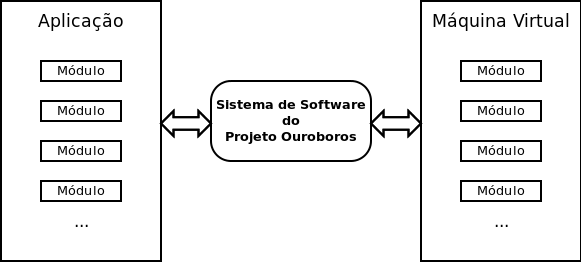
\includegraphics[width=.8\textwidth]{overview-simple.png}
      \caption{Esquematização bem simplificada do sistema.}
      \label{fig:overview-simple}
    \end{figure}

    Dessa forma, uma primeira ilustração bem simplificada da estrutura geral do
    nosso sistema é a representada na Figura \ref{fig:overview-simple}. O
    sistema Ouroboros será responsável por fornecer acesso aos módulos entre a
    aplicação e as máquinas virtuais. Então, a estrutura que queremos para o
    projeto deve levar isso em consideração, tratando os dois sentidos dessa
    interação como duas partes diferentes. Dessa forma, estabelecemos duas
    grandes funcionalidades no sistema: providenciar à aplicação a possibilidade
    de manipular os módulos das máquinas virtuais, e deixar os módulos da
    aplicação à disposição dos \script{s} . Esses processos são conhecidos como
    \textbf{incorporação}\footnote{Do inglês, ``\textit{embedding}''.} e
    \textbf{exportação}, respectivamente.

    \definicao{
      \vspace{-1.5em}
      \begin{enumerate}
        \item \textbf{Incorporação} é quando a aplicação programada na linguagem
              nativa pode acessar e manipular os elementos dos módulos da
              máquina virtual.
        \item \textbf{Exportação} é quando módulos da aplicação na linguagem
              nativa são registrados na máquina virtual de modo que os módulos
              desta possam usar funcionalidades daquela.
      \end{enumerate}
    }

    As duas próximas sessões explicarão como projetamos as partes do sistema
    que atenderão cada um desses requisitos. Nesse ponto vale à pena destacar
    um aspecto que ficou de lado até agora. Como o subtítulo desse trabalho
    indica, o propósito do sistema é não só integrar as ditas linguagens, como
    fazê-lo de maneira \textit{automatizada}. Até porque as APIs das máquinas
    virtuais por sí sós possuem seus próprios mecanismos de fornecer essas
    capacidades, mas são trabalhosas e específicas de usar. Isso também é
    considerado na elaboração da estrutura do projeto, como veremos a seguir.

  \section{Biblioteca de abstração de APIs de linguagens de \emph{script}.}
  \label{sec:estrutura:opa}
  
    Uma máquina virtual de uma linguagem de \script{} é implementada em uma outra
    linguagem, que chamamos de sua linguagem nativa. Enquanto nosso sistema trabalha
    com as linguagens nativas \C{} ou \CXX{}, podem existir implementações da máquina
    virtual para diversas linguagens. É comum a implementação de uma máquina virtual
    disponibilizar uma API para sua linguagem nativa, provendo funções, constantes
    e outros elementos para que a linguagem nativa consiga acessar e manipular a
    máquina virtual e seu conteúdo. Isso que representa, na prática, a interação do
    tipo (A).

    Infelizmente, para um usuário comum que está desenvolvendo um programa em
    linguagem nativa, usar a API de uma máquina virtual é normalmente uma tarefa
    difícil e trabalhosa pela complexidade da API e pelo tempo necessário para
    aprender a usá-la. Foi para resolver esse problema que desenvolvemos a
    biblioteca de abstração de APIs de linguagens de \script{}, também conhecida
    como \textit{libouroboros} ou simplesmente como \emph{Ouroboros Project API}
    (OPA).
    
    A libouroboros é a parte do nosso projeto que provê a interação do tipo (A),
    como explicada acima. Ela consiste em um conjunto de classes e funções em 
    \CXX{} que generalizam o meio com o qual se realiza diversas operações com 
    a API da linguagem de \script{}, como:
    \begin{itemize}
      \item carregar um \script{};
      \item executar uma função na máquina virtual;
      \item obter/configurar um objeto/atributo/valor na máquina virtual;
      \item converter valores entre linguagem nativa e a máquina virtual;
    \end{itemize}
    Uma parte dessa API é uma interface polimórfica que, ao ser implementada usando
    as rotinas da máquina virtual de uma linguagem de \script{}, possibilita que
    a \emph{libouroboros} reconheça e trabalhe com tal linguagem. Essa
    implementação deve satisfazer nossa interface, isso é, as operações
    descritas acima. A nossa API administrará as diversas implementações
    disponíveis apresentando ao usuário final da OPA apenas a interface
    unificada. Desse jeito, ele não precisa saber sobre esse gerenciamento
    interno, nem se preocupar com a API da linguagem de \script{}, a não ser que
    seja ele quem vá adicionar o suporte a ela no sistema.

    % TODO: Diagrama ilustrando relação da OPA com as APIs específicas de cada
    %       linguagem de script
    
    Por padrão, o projeto terá as implementações para \textit{Lua} e
    \textit{Python}, e portanto essas linguagens serão compatíveis com a OPA.
    
    %TODO: subsection: conversão de valores (entre linguagem nativa e máquina virtual)
    %TODO: subsection: virtualobj (possiveis subsubsection pra falar do encapsulamento do vdata, etc)
    %TODO: subsection: importação de um módulo de script para a linguagem nativa
  
  
  \section{Gerador de \emph{wrappers} e interfaces.}
  \label{sec:estrutura:opwig}

  %TODO: Explicar mais sobre a ideia geral da relação do tipo (B)

    Linguagens de \script{} possuem um mecanismo próprio para incluir módulos
    externos, eventualmente necessários à sua execução. Esses módulos podem ser
    definidos tanto em outros arquivos na mesma linguagem, quanto na linguagem
    nativa da máquina virtual. Nesse último caso, temos a relação do tipo (B). Ela
    exige que a linguagem nativa disponibilize certos dados seguindo um protocolo
    adequado. Infelizmente tal protocolo não só difere para cada linguagem de
    \script{} como também involve um trabalho repetitivo e maçante para ser utilizado. 

    %TODO: Detalhar esse processo repetitivo e maçante.
    
    Por isso, parte do nosso sistema é composto por um gerador automatizado de código fonte.
    Ele é responsável por criar o código necessário à devida exportação dos módulos 
    feitos na linguagem nativa. Além disso, ele processa código que o usuário fornecer na
    linguagem nativa para saber o conteúdo que deve aparecer no módulo exportado.
    Esse conteúdo é inserido no módulo através de \emph{wrappers}. Chamamos esse componente
    do sistema de \emph{Ouroboros Project Wrapper and Interface Generator} (OPWIG).
  
    %TODO: subsection: parser
    %TODO: subsection: code generator
    %TODO: subsection: wrapper explanation 
  
  \section{Integrando e entregando tudo para o usuário.}
  \label{sec:estrutura:integration}

    Isso será escrito na versão final da monografia.
